% !TeX root = main.tex

\section{Linear time scaling}

\subsection{Rule-based linear time scaling}

We use the scaling factor as a function of the simulation time, given by $s(t) = a + bt$. The scaling is done as in constant time scaling case. The results are shown in figure \ref{fig:rb-lts-exp1-graphs}. The snippets from simulation are shown in figure \ref{fig:rb-lts-exp1}.

It is interesting to note that the scaling factor plot (figure \ref{fig:sfig-rb-lts-e1-ts}) shows a straight line in between the scaling times, while the time plot (on its left) shown a parabolic joint (because of accelerating time, as change is linear in time). The code to generate these figures is given in appendix \ref{app:nh-rb-lts-code}.

\begin{figure}[ht]
    \centering
    \begin{subfigure}[b]{0.49\textwidth}
        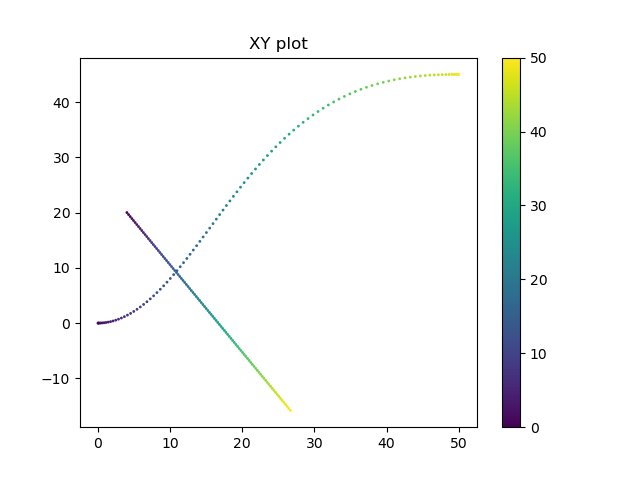
\includegraphics[width=\textwidth]{rb-lts-xy.png}
        \caption{XY plots}
        \label{fig:sfig-rb-lts-e1-xy}
        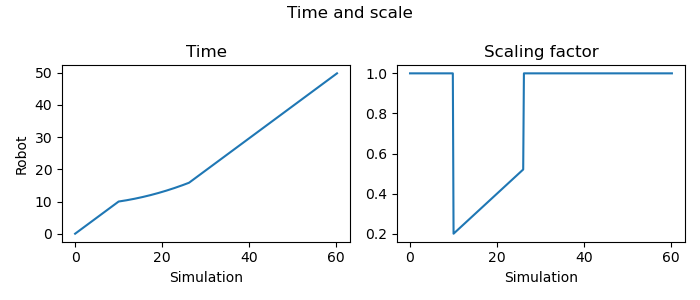
\includegraphics[width=\textwidth]{rb-lts-tscales.png}
        \caption{Time scaling}
        \label{fig:sfig-rb-lts-e1-ts}
    \end{subfigure}
    \begin{subfigure}[b]{0.49\textwidth}
        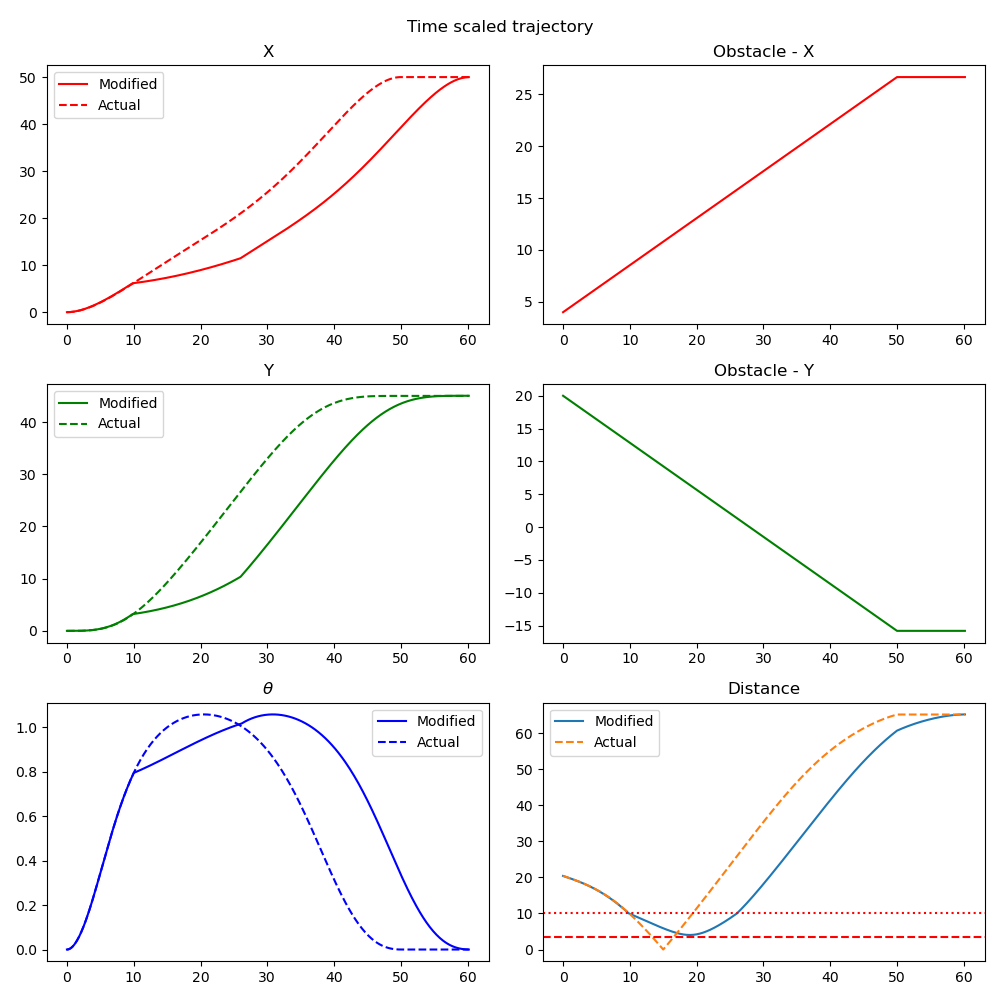
\includegraphics[width=\textwidth]{rb-lts-trajs.png}
        \caption{Time scaled results}
        \label{fig:sfig-rb-lts-e1-fgr}
    \end{subfigure}
    \caption{Rule-based Linear time scaling}
    \label{fig:rb-lts-exp1-graphs}
    \small
        The distance plot is shown in the bottom right of \ref{sub@fig:sfig-rb-lts-e1-fgr}. As seen, the time scaling gets activated at the thin red horizontal line (detection distance) and a collision is avoided (the distance plot does not cross the thick horizontal red line). See the slope and the scaling factor change in \ref{sub@fig:sfig-rb-lts-e1-ts} (notice the linear slope, with time as parabolic). The original (colliding) trajectories are shown in \ref{sub@fig:sfig-rb-lts-e1-xy}.
\end{figure}

\begin{figure}[ht]
    \centering
    \begin{subfigure}[b]{0.3\textwidth}
        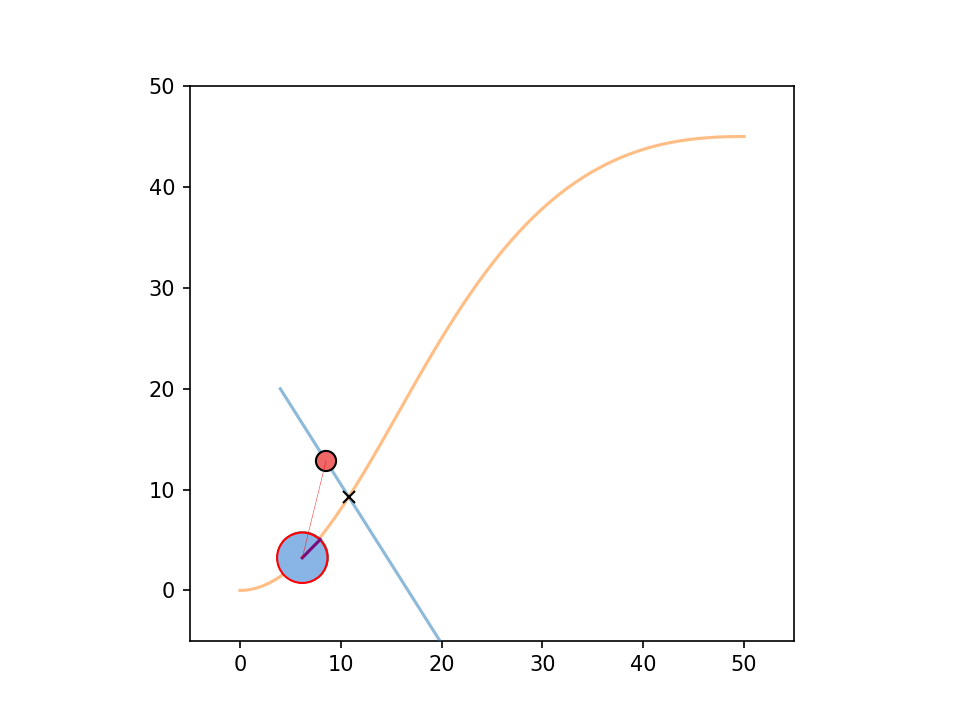
\includegraphics[width=\textwidth]{res3-ts-start.png}
        \caption{Start}
    \end{subfigure}
    \begin{subfigure}[b]{0.3\textwidth}
        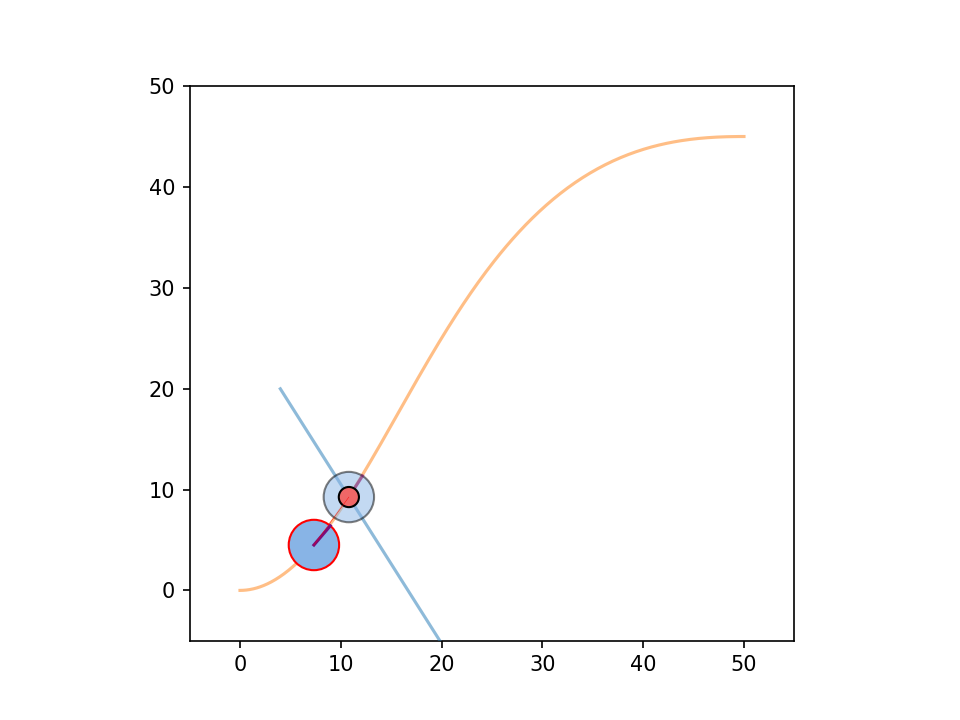
\includegraphics[width=\textwidth]{res3-ts-colav.png}
        \caption{Collision avoidance}
    \end{subfigure}
    \begin{subfigure}[b]{0.3\textwidth}
        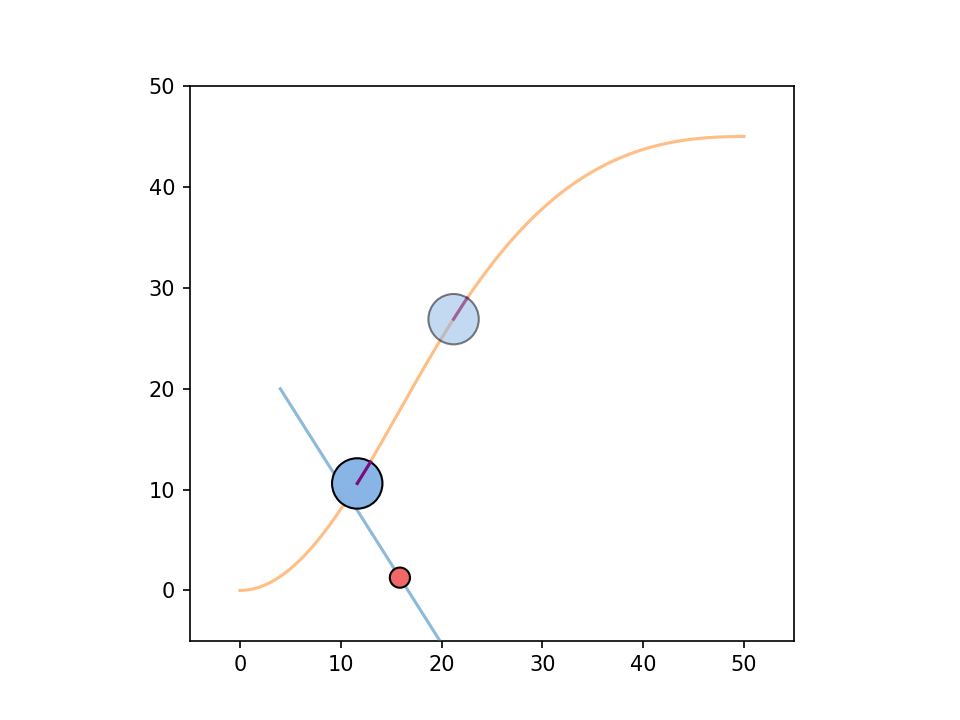
\includegraphics[width=\textwidth]{res3-ts-end.png}
        \caption{End}
    \end{subfigure}
    \caption{Rule-based - Linear time scaling - Video snaps}
    \label{fig:rb-lts-exp1}
    \small
        The simulation is available as \texttt{rb\_lts\_exp1.avi} in the \href{https://iiitaphyd-my.sharepoint.com/:f:/g/personal/avneesh_mishra_research_iiit_ac_in/Er_wRqK4hxVLjVdL56rfDxYBKr9PPed1laN48hLgLisf4w}{shared OneDrive folder}.
\end{figure}
